\label{sec:pipeline}

In this section the pipeline is presented, which allows to convert an image of an \ac{ECD} into the LTspice schematic file format.
To fully convert the \ac{ECD} from the \ac{IDom} into the \ac{LDom} the following needed conditions have been identified:

\begin{itemize}
    \item the class and position of the \acp{ECC}
    \item the text and position of the annotations as well as the annotation mapping (to which \ac{ECC} belongs this annotation)
    \item the connections between the \acp{ECC}
    \item the conversion into the LTspice schematic file
\end{itemize}

The above points are all embedded into a three-stage pipeline, which will be presented throughout this section.

\subsubsection{Recognition}

Predicting the class and position of an object can essentially be formulated as an object detection problem.
Various object detection networks exist, which could be used for this task.
In this thesis the presented \ac{YOLOv4}-Tiny (section \ref{sec:yolo}), or just \ac{YOLO} is used to predict the \acp{ECC}, \ac{ECC}-annotations (arrows for sources) and the text annotations in the \ac{IDom}.
\ac{YOLO} was chosen since it has a good compromise between network size and classification performance.

Furthermore, the pipeline also utilizes segmentation to segment the circuit.
Segmentation is needed because the topology building step, which will be described next requires a clean mask of the circuit.
The initial clean mask was created using image binarization.
While the topology building worked for circuits with white background it failed for circuits with checkered background.
Therefore, the \ac{MUnet} (section \ref{sec:mobilenetv2_unet}) is used to segment a circuit in the \ac{IDom}.
The network predicts a binary classification output in the form background / not background, where everything which is unrelated to the \ac{ECD} is considered background.
Note that the network was trained for both checkered and uncheckered backgrounds, such that it can be applied on both types of images.
Again, \ac{MUnet} was chosen, since it is a lightweight network with appropriate performance, able to be used on mobile devices.

An example prediction of both networks can be seen in figure \ref{fig:example_predictions}.

\begin{figure}
\begin{center}
    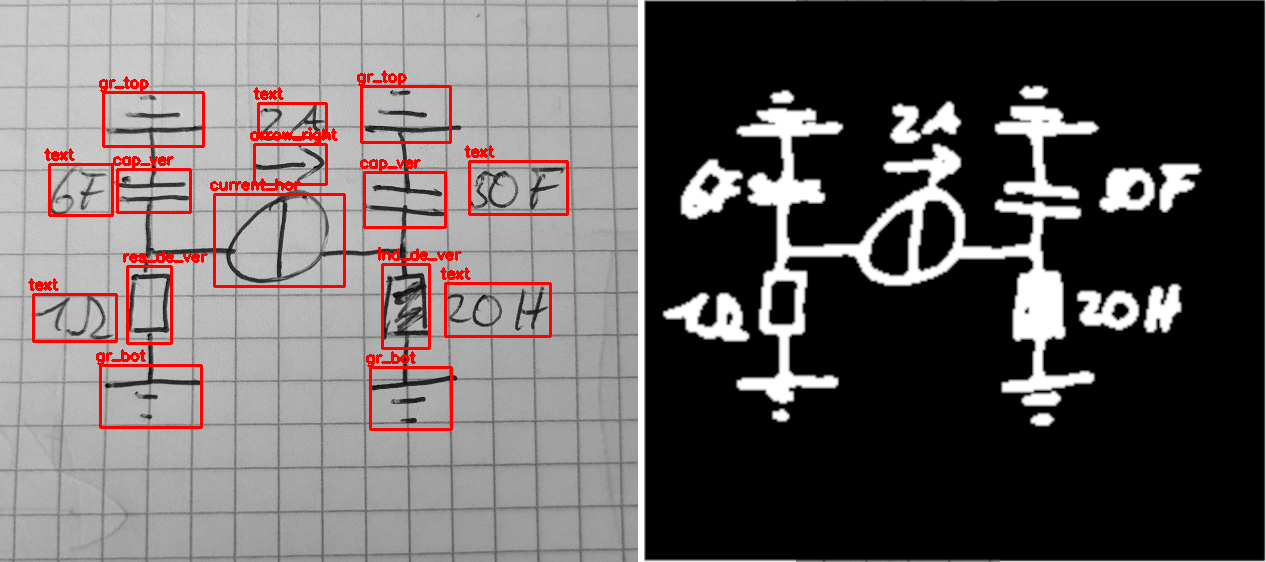
\includegraphics[width=16cm]{imgs/pipeline/combined_pred.png}
    \caption{Example predictions of YOLO (left) and \ac{MUnet} (right). YOLO predicts a bounding box around each component with its corresponding class, while \ac{MUnet} predicts a segmentation mask a binary fashion of the whole \ac{ECD} drawing, including \ac{ECC} annotations. Primary segmentation is needed to remove the checkered background from the image.}
    \label{fig:example_predictions}
\end{center}
\end{figure}

\subsubsection{Topology Creation}

The next step in the pipeline is the identification of the connections between the \acp{ECC}, such that the wires from the \ac{IDom} can be transformed into the \ac{LDom}.
In an abstract form this is topology creation.
This step does not take into account the spatial positions of the components, but only the semantics of the circuit.
In the following the algorithm is presented, which takes as input the predicted bounding boxes and the segmentation mask of the circuit and produces the topology of the circuit.
The algorithm utilizes various OpenCV algorithms, which are first briefly explained.

\textbf{Adaptive Binary Thresholding} TODO? maybe I won't use it any more

\textbf{Connected Components Labeling} by Grana et al. \cite{cca} is an 8-way connectivity algorithm used to label blob like regions in a binary image.
In the topology creation process it is used to identify the wires.

\textbf{Morphological Operations} like erosion, dilation or the combinations of those like opening and closing \cite{cv}, are used to filter the used binary images and to refine results obtained from various sources in the pipeline.

After the basic methods were presented now the algorithm can be explained.
The algorithm receives as input the predicted bounding boxes and the segmentation mask of the circuit.

\begin{enumerate}
    \item Copy the \textbf{SegmentationMask} $\in \{0,1\}^{h \times w}$  into \textbf{WiresOnly}. Iterate over the bounding boxes (bbox $\in \{x1, y1, x2, y2, class\}$, where $(x1, y1)$ represent the upper left corner of the bounding box and $(x2, y2)$ the lower right) and remove every pixel in \textbf{WiresOnly}, which is included in a bounding box. Only the wires remain now.
    \item Perform morphological closing on \textbf{WiresOnly} to close up small holes in the wires.
    \item Apply connected components labeling on \textbf{WiresOnly} to label the separate wire blobs resulting in \textbf{WiresLabeled}.
    \item Create a matrix \textbf{BBoxMask} of zeros with the size of \textbf{WiresOnly}. Iterate over the bounding boxes and populate \textbf{BBoxMask} with rectangles with a thin border created from the bounding box coordinates.
    \item Apply the and-operator on \textbf{WiresLabeled} and \textbf{BBoxMask} and receive the intersections, where a wire is intersecting the border of a bounding box. Store the result in \textbf{Intersections}.
    \item Initialize a dictionary \textbf{Topology} and populate it by iterating over \textbf{Intersections} and for each intersection index check the connected components label at this index create an entry in \textbf{Topology} with an empty array.
    \item Iterate over each intersections index and find the bounding box which is ``involved'' in this intersection. A bounding box is ``involved'', when intersection index $\in$ bounding box border and the class of the bounding box is an \ac{ECC}.
    \item Find the orientation of the intersection. Orientation refers to the connection orientation relative to the bounding box, i.e. is the intersection at the top, bottom, left or right border.
    \item Get the connected components label at the intersection index and add a tuple of (bounding box index, orientation) at the respective spot in the \textbf{Topology} if this index with this orientation is not present.
    \item After the initial \textbf{Topology} is build, iterate over it and remove each connected component label, where the involved bounding boxes array has $size = 1$ and the involved bounding box has a contradictory orientation in relation to the predicted class, i.e. classes predicted with vertical orientation can only have a connection at the top or bottom, classes predicted with horizontal orientation can only have a connection left or right.
    \item Return the \textbf{Topology}
\end{enumerate}

\subsubsection{Annotation Matching}

In this thesis different annotations are used.
Arrow annotations are only used for voltage and current sources to indicate the direction of the potential difference as well as the current flow, respectively.
On the other side textual annotations can be applied to any type of an \ac{ECC}.
To fully reflect the circuit in the \ac{LDom} annotations have to be matched against their respective \ac{ECC}.
The algorithm used in this thesis is presented in algorithm \ref{alg:annotation_matching}, it takes as input a list of arrow bounding boxes, a list of text bounding boxes and a list of \acp{ECC}.
An annotation is matched against an \ac{ECC} using a simple brute force nearest neighbor approach, based on the center distance of the bounding boxes to match.
Brute force in the sense that every annotation will get matched against an \ac{ECC} without considering that the distance between annotation and \ac{ECC} is maybe way too big, like it would be the case for example when a \ac{FP} annotation is predicted, it certainly will get matched.
Multiple annotations are also possible with this algorithm, but when this occurs the one with the smallest distance is taken and the other match is ignored.

\begin{algorithm}[caption={Annotation Matching TODO caption to bottom and format}, label={alg:annotation_matching}]
input:  $A = \{a_1, ..., a_n\}$, $T = \{t_1, ..., t_m\}$, $E = \{e_1, ..., e_o\}$
        $A$: list of predicted arrow bounding boxes
        $T$: list of predicted text bounding boxes
        $E$: list of predicted ECC bounding boxes
output: $A_m = \{(a_1, e_i), ..., (a_n, e_j)\}$
        $T_m = \{(t_1, e_x), ..., (t_m, e_y)\}$
        $A_m$: list of arrow bounding boxes matched against source bounding boxes
        $T_m$: list of text bounding boxes matched against ECC bounding boxes

begin
    $A_m = \{\}$
    foreach $a$ in $A$; do
        $distances = \{\}$

        $a_{center}$ = get_bounding_box_center($a$)
        foreach $e$ in $E$; do
            if is_source_type($e$); then
                $e_{center}$ = get_bounding_box_center($e$)
                $dist$ = euclidean_distance($a_{center}$, $e_{center}$)
                $distances$ $\gets$ $distances + (dist, a, e)$
            end
        end

        $min_{dist}$, $a_{matched}$, $e_{matched}$ = sort_ascending_by_distance($distances$)[0]
        $A_m = A_m \gets (a_{match}, e_{match})$
    end

    $T_m = \{\}$
    foreach $t$ in $T$; do
        $distances = \{\}$

        $t_{center}$ = get_bounding_box_center($t$)
        foreach $e$ in $E$; do
            $e_{center}$ = get_bounding_box_center($e$)
            $dist$ = euclidean_distance($t_{center}$, $e_{center}$)
            $distances$ $\gets$ $distances + (dist, t, e)$
        end

        $min_{dist}$, $t_{matched}$, $e_{matched}$ = sort_ascending_by_distance($distances$)[0]
        $T_m = T_m \gets (t_{match}, e_{match})$
    end

    return $A_m$, $T_m$
end
\end{algorithm}


\subsubsection{LTspice Conversion}

The last step in the proposed pipeline is the embedding of the gathered information into the LTspice schematic file.

TODO not 100\% sure how this will be written
